\begin{onehalfspace}

Stabiliti gli strumenti, questo capitolo definisce il disegno sperimentale della prima fase. Il contratto separa la correttezza ideale dell'algoritmo, il modello illustrativo di rumore e le regole del confronto statistico. Gli esiti numerici non fanno parte della metodologia: le tabelle con $\bar M$, $\rho$ e p-value nel Capitolo~\ref{chap:risultati} sono estratte esclusivamente dagli artefatti schema~2 prodotti con il circuito N15 corretto.

% -----------------------------------------------
\section{Obiettivi della Parte Sperimentale}
\label{sec:obiettivi_sperimentali}

Il primo obiettivo è costruire una \textbf{baseline riproducibile}. Il Metodo~1 esamina la misura più frequente dell'istogramma (TOP-1), applica frazioni continue e \ac{GCD} e ripete il campionamento fino al successo o al budget massimo. Il secondo obiettivo è confrontare, sullo stesso dato, due estensioni: TOP-4 senza apprendimento e il Metodo~2, nel quale un classificatore decide se attivare la ricerca TOP-4. Questa terna permette di distinguere il contributo della ricerca multi-candidato da quello del modello appreso.

La campagna rumorosa è limitata a $N=15$, $a=7$, con due preset uniformi illustrativi: riferimento e stress. I moltiplicatori di Beauregard per $N=21$ e $N=35$ sono invece validati idealmente e sottoposti ad audit di risorse, ma esclusi dalle simulazioni rumorose complete. La separazione evita di trasformare un limite computazionale del simulatore in un risultato sulla probabilità di successo dell'algoritmo.

% -----------------------------------------------
\section{Architettura del Pipeline Sperimentale}
\label{sec:architettura}

Il sistema è strutturato come una pipeline a tre stadi, illustrata in Figura~\ref{fig:pipeline_architettura}.

\begin{figure}[H]
\centering
\resizebox{\textwidth}{!}{%
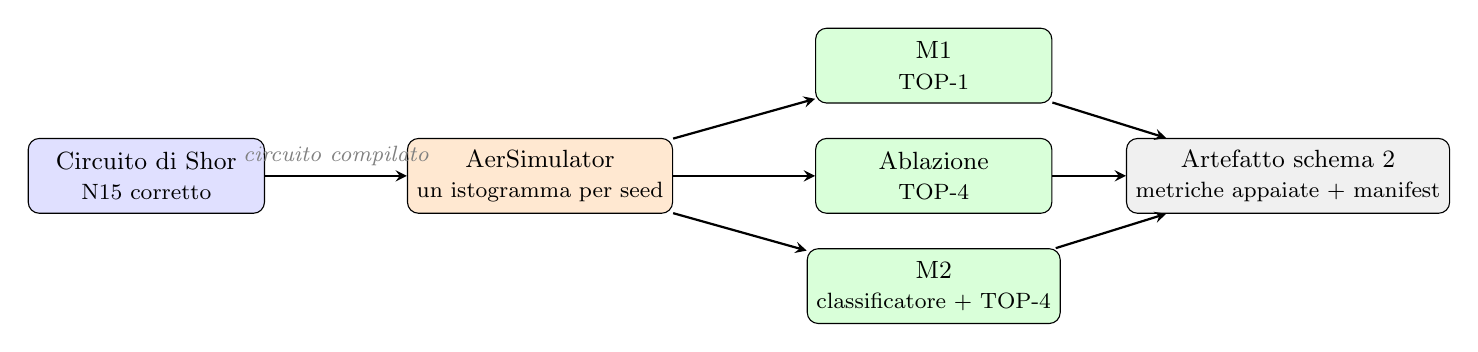
\begin{tikzpicture}[
    box/.style     = {rectangle, draw, rounded corners=4pt,
                      minimum width=3.0cm, minimum height=0.95cm,
                      align=center, font=\small},
    arrow/.style   = {->, thick, >=stealth},
    lbl/.style     = {font=\footnotesize\itshape, text=gray}
]
\node[box, fill=blue!12]   (shor)  at (0,    0)   {Circuito di Shor\\{\footnotesize N15 corretto}};
\node[box, fill=orange!18] (noise) at (5.0,  0)   {AerSimulator\\{\footnotesize un istogramma per seed}};
\node[box, fill=green!15]  (m1)    at (10.0, 1.4) {M1\\{\footnotesize TOP-1}};
\node[box, fill=green!15]  (mt4)   at (10.0, 0)   {Ablazione\\{\footnotesize TOP-4}};
\node[box, fill=green!15]  (m2)    at (10.0,-1.4) {M2\\{\footnotesize classificatore + TOP-4}};
\node[box, fill=gray!12]   (out)   at (14.5, 0)   {Artefatto schema 2\\{\footnotesize metriche appaiate + manifest}};
\draw[arrow] (shor)  -- node[above, lbl]{circuito compilato} (noise);
\draw[arrow] (noise) -- (m1);
\draw[arrow] (noise) -- (mt4);
\draw[arrow] (noise) -- (m2);
\draw[arrow] (m1)  -- (out);
\draw[arrow] (mt4) -- (out);
\draw[arrow] (m2)  -- (out);
\end{tikzpicture}%
}
\caption[Pipeline sperimentale appaiata]{Pipeline versione~2. Per ogni coppia (replica, iterazione) Aer genera un solo istogramma, poi riusato dalle tre strategie. Il confronto non introduce quindi differenti realizzazioni Monte Carlo.}
\label{fig:pipeline_architettura}
\end{figure}

\textbf{Stadio 1 --- circuito.} Per $N=15$ il moltiplicatore controllato implementa $y\mapsto 7y\bmod15$ ripetendo l'operazione elementare esattamente \texttt{power} volte. Il circuito viene compilato con Qiskit~2.5, \texttt{optimization\_level=2}, seed del transpiler fissato e base nativa esplicita \texttt{rz/sx/x/cx}. Il manifest della configurazione di riferimento registra profondità 412, 224 porte \texttt{cx}, conteggi completi delle istruzioni e hash SHA-256 della netlist. La simulazione ideale valida il periodo e l'estrazione dei fattori in termini probabilistici; non si assume che ogni singolo shot produca necessariamente un fattore.

\textbf{Stadio 2 --- rumore.} Il circuito compilato viene eseguito con un noise model uniforme e controllabile. I due preset servono a studiare il comportamento del metodo, non a emulare o calibrare una specifica QPU. Ogni artefatto conserva sia i parametri sia il manifest del circuito, così risultati ottenuti con revisioni differenti non possono essere combinati inavvertitamente.

\textbf{Stadio 3 --- analisi.} M1, TOP-4 e M2 ricevono il medesimo istogramma. Un ordinamento deterministico risolve i pareggi di frequenza mediante una priorità SHA-256 costruita da seed e bitstring: l'ordine non dipende dall'inserimento nel dizionario e non favorisce sistematicamente bitstring alte o basse.

% -----------------------------------------------
\section{Tecniche di Mitigazione del Rumore: Analisi e Scelte Implementative}
\label{sec:mitigazione_scelte}

\subsection{Transpilazione e Riduzione della Profondità}
\label{subsec:transpilazione}

Il gate set è fissato a \texttt{rz/sx/x/cx} prima dell'esecuzione. Questa scelta rende esplicite le sole istruzioni a cui il noise model può essere associato ed evita che porte composite sopravvivano fuori dal contratto. Per $N=15$ la compilazione globale di riferimento produce 224 \texttt{cx} e profondità 412; questi valori sono proprietà della coppia (circuito, versione e opzioni del transpiler), perciò vengono verificati e registrati anziché assunti dal sorgente astratto.

Per $N=21$ e $N=35$ si usa la costruzione aritmetica reversibile di Beauregard. I test ideali coprono le truth table sui sottospazi validi, la pulizia di registro ausiliario e ancilla e il comportamento QPE. La compilazione completa $N=21$, $a=2$, $n_{\text{count}}=8$, livello~2, conta 21\,036 \texttt{cx} e ha profondità 23\,081. Il proxy registrato a $\lambda=10^{-3}$ è $7.2379\times10^{-10}$; è un indicatore circuitale di accumulo, non una stima di $P(\text{successo})$. Il costo giustifica l'esclusione di N21/N35 dalle campagne rumorose, pur lasciandone valida la verifica ideale.

\subsection{Modello di Rumore Uniforme}
\label{subsec:noise_uniforme}

Le rotazioni \texttt{rz} sono trattate come cambi di frame virtuali, con durata ed errore nulli. I gate \texttt{sx} e \texttt{x} hanno durata 50\,ns; \texttt{cx} ha durata 300\,ns. Su \texttt{sx/x} si compongono il canale depolarizzante a un qubit e il rilassamento termico della durata 1Q; su \texttt{cx} si compongono i corrispondenti canali a due qubit e il rilassamento per 300\,ns. Il readout è modellato da una matrice di confusione simmetrica. Non vengono associati errori a \texttt{rz}, né a istruzioni fuori dalla base.

Nel costruttore Aer, il parametro passato a \texttt{depolarizing\_error} è $\lambda$ nella mappa
\begin{equation}
    \mathcal{E}(\rho)=(1-\lambda)\rho+\lambda\frac{I}{2^n}.
\end{equation}
Per un gate a due qubit, la probabilità aggregata della componente di Pauli non identità nella rappresentazione equivalente è $15\lambda/16$. Di conseguenza, per i 224 \texttt{cx} del circuito N15 si usa esclusivamente il proxy
\begin{equation}
    P_{\text{no-Pauli-2Q}}=\left(1-\frac{15\lambda}{16}\right)^{224}.
    \label{eq:proxy_no_pauli_2q}
\end{equation}
Questa quantità non comprende rilassamento, errori 1Q o readout e, soprattutto, non è la probabilità di successo dell'algoritmo di Shor.

\subsection{Livello di Misura: Mitigazione degli Errori di Readout}
\label{subsec:readout_mitigation}

Il contratto base non applica un'inversione post-hoc della matrice di assegnazione. Il parametro $p_{\text{ro}}$ viene invece variato nella campagna parametrica, mantenendo il resto del preset costante. Le conclusioni quantitative sull'impatto del readout provengono dall'artefatto schema~2 corrente; le campagne antecedenti alla correzione del circuito non vengono riutilizzate.

\subsection{Zero-Noise Extrapolation}
\label{subsec:zne}

La \ac{ZNE} resta un termine di confronto metodologico. I fattori di scala moltiplicano i parametri del noise model, mentre il costo in shot e le trasformazioni dell'istogramma vengono registrati separatamente. Il suo effetto su $\bar M$ e la significatività del confronto sono valutati sotto lo stesso circuito e lo stesso schema statistico della baseline; l'esito è riportato nell'Appendice~\ref{app:parametrica}.

\subsection{Analisi di Sensibilità}
\label{subsec:sensitivity}

La campagna parametrica adotta una variazione singola rispetto al preset di riferimento e comprende $K$, $\lambda_{2q}$, shots, $T_1/T_2$, $\lambda_{1q}$ e $p_{\text{ro}}$, oltre alle griglie congiunte dichiarate nel manifest. La base circuitale resta invariata. Le tabelle correnti provengono dalla rigenerazione schema~2; gli artefatti storici precedenti alla correzione di \texttt{c\_amod15} non sostengono conclusioni scientifiche.

\subsection{Scelta Adottata: Classificatore come Filtro}
\label{subsec:scelta_ml}

Il classificatore riceve il vettore normalizzato delle $2^{n_{\text{count}}}$ frequenze. La generazione del dataset calcola nello stesso passaggio sia l'etichetta TOP-1 sia l'etichetta TOP-16, così l'effetto della definizione di target è auditabile senza cambiare i campioni. Il modello ammesso nella pipeline M2 è quello con \texttt{label\_top\_k=1} e manifest compatibile; TOP-16 resta un'analisi di sensibilità dell'etichetta. Dopo l'accettazione del classificatore, M2 tenta i primi quattro candidati dello stesso ordinamento usato dall'ablazione TOP-4.

% -----------------------------------------------
\section{Il Metodo 1: Baseline TOP-1}
\label{sec:metodo1}

Per ogni iterazione il Metodo~1:
\begin{enumerate}
    \item riceve l'istogramma comune della replica;
    \item seleziona il primo candidato nell'ordinamento frequenza--SHA-256;
    \item stima il periodo con frazioni continue e verifica i fattori non banali;
    \item in caso di fallimento procede all'istogramma successivo, fino a $M_{\max}$.
\end{enumerate}

Il seed Aer è separato fra iterazioni di più del numero di shot, secondo la formula dichiarata nell'implementazione. Questo evita la sovrapposizione quasi completa dei flussi pseudo-casuali prodotta da semi consecutivi.

% -----------------------------------------------
\section{Il Metodo 2 e il Disegno Appaiato}
\label{sec:metodo2}

TOP-4 prova, in ordine, fino a quattro candidati dello stesso istogramma. M2 applica prima il classificatore e, soltanto se il gate è positivo, esegue la medesima ricerca TOP-4. Per ciascuna replica si registra la prima iterazione di successo di ogni strategia. Un mancato successo entro $M_{\max}$ è codificato con la sentinella $M_{\max}+1$, mantenendolo distinto da un successo all'ultima iterazione.

Il calendario di seed e gli istogrammi sono comuni a tutte le strategie. I confronti M1$>$TOP-4 e M1$>$M2 usano il Wilcoxon appaiato unilaterale con gestione degli zeri secondo Pratt; il confronto TOP-4--M2 è bilaterale. Medie, deviazioni e tassi di successo sono statistiche descrittive; il vettore completo con le sentinelle è usato per l'inferenza. L'output JSON schema~2 include input, seed, vettori appaiati, test, versione del software e manifest/hash della compilazione.

\end{onehalfspace}
